\documentclass{report}
\usepackage[T1]{fontenc} % Fontes T1
\usepackage[utf8]{inputenc} % Input UTF8
\usepackage[backend=biber, style=ieee]{biblatex} % para usar bibliografia
\usepackage{csquotes}
\usepackage[portuguese]{babel} %Usar língua portuguesa
\usepackage{blindtext} % Gerar texto automaticamente
\usepackage[printonlyused]{acronym}
\usepackage{hyperref} % para autoref
\usepackage{graphicx}
\usepackage{indentfirst} % indentação da primeira linha
\graphicspath{{imagens/}} 

\bibliography{bibliografia}


\begin{document}
%%
% Definições
%
\def\titulo{Formula 1}
\def\data{19/12/2021}
\def\autores{Beatriz Ferreira, Tomás Fonseca}
\def\autorescontactos{(107214) beatriz.ferreira@ua.pt, (107245) tomasfonseca14@ua.pt}
\def\departamento{DETI}
\def\empresa{Universidade de Aveiro}
\def\logotipo{ua.pdf}
%
%%%%%% CAPA %%%%%%
%
\begin{titlepage}

\begin{center}
%
\vspace*{50mm}
%
{\Huge \titulo}\\ 
%
\vspace{10mm}
%
{\Large \empresa}\\
%
\vspace{10mm}
%
{\LARGE \autores}\\ 
%
\vspace{30mm}
%
\begin{figure}[h]
\center
\includegraphics{\logotipo}
\end{figure}
%
\vspace{30mm}
\end{center}
%
\begin{flushright}
\end{flushright}
\end{titlepage}

%%  Página de Título %%
\title{%
{\Huge\textbf{\titulo}}\\
{\Large \departamento\\ \empresa}
}
%
\author{%
    \autores \\
    \autorescontactos
}
%
\date{\data}
%
\maketitle

\pagenumbering{roman}

%%%%%% RESUMO %%%%%%
\begin{abstract}


Este projeto tem como objetivo abordar o tema sobre a segurança nos carros de Formula 1, como foi evoluindo ao longo das décadas e qual o impacto dessa evolução no mundo viação civil.
 Iremos abordar no primeiro capítulo como começou a Formula 1, as equipas que a constituíam, a historia das cores utilizadas nos carros e a sua evolução nas primeira década.
 No segundo capítulo abordaremos a falta de segurança que existia nos primórdios da Formula 1, o número de mortes registadas no seu começo e as razões pela qual a taxa de mortalidade seria tão elevada neste desporto.
No capítulo três vamos discutir o estado da Formula 1 atualmente, a razão pela qual se tornou um desporto mais seguro e em que medida, isso tornou o espírito de competitividade mais elevado entre os pilotos.
No capítulo quatro vamos apresentar quais foram os avanços tecnológicos mais importantes que tornaram a Formula 1 mais segura, competitiva, apelativa e intensa, aprofundando cada um destes. 
No último capítulo vamos falar sobre as inovações da Formula 1 utilizadas atualmente no mundo da viação civil.


O projeto termina concluindo com o quanto a Formula 1 evoluiu e o quão seguro o desporto se tornou a partir do ano de 1950 até atualmente.

\end{abstract}


\tableofcontents
% \listoftables     % descomentar se necessário
% \listoffigures    % descomentar se necessário


%%%%%%%%%%%%%%%%%%%%%%%%%%%%%%%
\clearpage
\pagenumbering{arabic}

%%%%%%%%%%%%%%%%%%%%%%%%%%%%%%%%
\chapter{Introdução}
\label{chap.introdução}

\begin{figure}[h]
\center % Centra as imagens
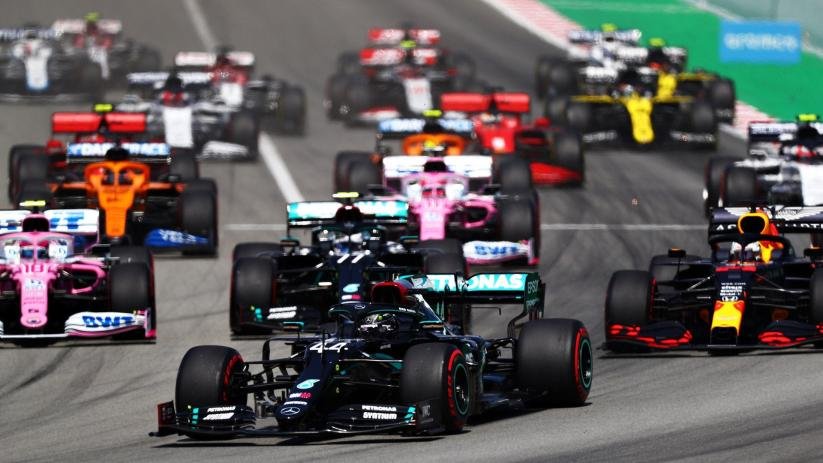
\includegraphics[height=150pt]{formula1}
\caption{Formula 1}
\label{fig:formula1}
\end{figure}

A \ac{f1} é uma das competições desportivas mais assistidas no mundo com um recorde de audiência na TV de 1,92 bilhão em 2019 (Formula 1, 2020). Tendo começado em 1950, agora é televisionado e ocorrem corridas em mais de 20 países todos os anos (Gutiérrez e Lozanzo, 2012). Embora o público principal da \ac{f1} seja europeu, de acordo com dados de mercado monitorizado pela Nielsen, recentemente a base de fãs da \ac{f1} cresceu significativamente para outras partes do mundo, como a China, Brasil, México, EUA e Índia (Formula 1, 2020). 


Em comparação com outros eventos de corrida de carros, como NASCAR e IndyCar, \ac{f1} é considerada o auge da inovação na indústria dos automóveis devido ao seu nível de sofisticação da tecnologia, localização geográfica, diversidade de circuitos, pilotos, equipas e a construção dos seus carros (Gutiérrez e Lozanzo, 2012).


 Atualmente, 10 equipas (oficialmente conhecidas como construtores) participam na competição durante um período de aproximadamente nove meses por temporada do calendário. Os construtores são formalmente definidos como empresas que “integram os vários componentes de domínios de conhecimento para construir o veículo final de automobilismo” (Pesquisa de automobilismo Associates, 2003). Cada construtor desenvolve e constrói dois carros de forma a competir durante as 21 corridas (cada uma oficialmente designada por “Grand Prix”) que constituem a temporada com esses mesmos. 
 
 
 As equipas esforçam-se para marcar o maior número de pontos com base na sua posição final numa corrida, para disputar dois títulos, a saber, o campeonato de pilotos e o campeonato de construtores (com o último sendo o mais importante para a equipa e o anterior mais importante para os pilotos). A fim de garantir uma competição justa e segura, a \ac{fia} é responsável por estabelecer e executar os regulamentos esportivos da \ac{f1} (Fédération Internationale De L’Automobile, 2020).


Desde 1950 até aos dias de hoje nunca se pensou que a \ac{f1} progredisse tanto, de pilotos com capacete de pano a competir em torno de uma base aérea em desuso ao desporto mais tecnologicamente avançado do mundo. Neste sentido, a \ac{f1} é a que mais contribuiu para o desenvolvimento em geral da viação civil. Tendo em conta as afirmações e os factos anteriormente apresentados, este projeto centrar-se-á na seguinte questão:
\begin{center}
“O quanto a Formula 1 evoluiu em 71 anos, e qual foi o seu impacto na viação civil?”
\end{center}


\chapter{História da Formula 1}
Emocionante, glamoroso e rápido. A \ac{f1} é o desporto mais emocionante 
do mundo, com 500 milhões de fãs, todos focados nos 20 pilotos e 10 equipas que disputam a glória de vencer o Campeonato Mundial.
Como surgiu a \ac{f1}?


No início do século XX a competição desportiva expandia-se por todo o mundo, entre os desportos dava-se maior destaque para o automobilismo, onde os pilotos guiavam carros especificamente modificados para a velocidade em circuitos isolados procurando ver quais destes seriam os melhores. Algumas organizações promoviam corridas prolongadas como as 500 milhas de Indianápolis nos Estados Unidos e um campeonato de corridas europeias. 
Houve uma pausa durante os anos (1939-1945) estas competições foram interrompidas devido á grande guerra mundial. Após o fim desta guerra, a \ac{fia} decidiu criar uma categoria que visava um campeonato mundial.


Em 13 de maio de 1950, em Silverstone na Inglaterra, surgiu então a \ac{f1}. O que viria a ser como o maior e mais caro desporto mundial à face da Terra. Na sua inauguração a \ac{f1} contou com 21 carros fornecidos por 5 equipas (Alfa Romeo, Alta, ERA, Maserati e Talbolt), pilotos de 7 países (Argentina, Escócia, França, Inglaterra, Irlanda, Itália e Tailândia) e um público com mais de 100.000 pessoas. A corrida teve uma duração de 2 horas e 13 minutos que se traduziu em 70 voltas ao circuito inglês, e a vitória do piloto da Alfa Romeo, Nino Farina, como podemos ver na \autoref{fig:Primeira corrida de Fórmula 1}. Poucos carros terminaram a corrida que teve pouca competitividade e o entretenimento apenas daqueles que já entendiam de \ac{f1}, mas que viria a crescer em breve.\\[2cm]
\begin{figure}[h]
\center % Centra as imagens
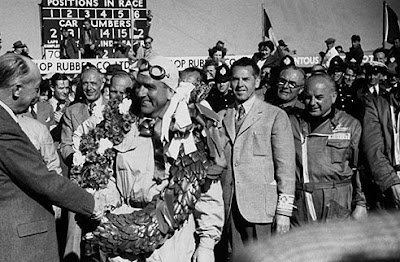
\includegraphics[height=150pt]{Primeira corrida de Formula 1}
\caption{Primeiro Grande Prêmio de Fórmula 1 e seu vencedor Nino Farina}
\label{fig:Primeira corrida de Formula 1}
\end{figure}
 
\section{Cores e os seus significados} 

As cores tradicionais dos carros no início da \ac{f1} eram as seguintes:

\begin{itemize}
\item verde para as equipes inglesas;
\item vermelho para as italianas;
\item azul para as francesas;
\item amarelo para as equipes belgas;
\item branco para as alemãs, que mais tarde adotariam a cor prata;
\item branco seria dos americanos, que eram vermelhos, porém os italianos adotariam essa cor.
\end{itemize}


 A cor prata passou a ser a cor tradicional dos carros de corrida alemães e por isso ganharam o apelido de Flechas Prateadas (Mercedes-Benz).
 O vermelho, inicialmente adotado pelos americanos na Copa Gordon Bennett, passou para os italianos após uma corrida entre Pequim e Paris, datada de 1907, vencida por uma equipe italiana. Na ocasião, a dupla formada pelo príncipe Scipione Borghese e pelo co-piloto Ettore Guizzardi cruzou a linha de chegada em primeiro lugar com um carro Italiano pintado em vermelho. Como as cores da Copa Gordon Bennett não era obrigatórias (e até hoje, trata-se de uma convenção histórica), os italianos passaram a adotar o vermelho, que logo virou tradição. Embora seja comum ouvir a expressão “vermelho Ferrari”, a cor é adotada também por outras equipes italianas.\\[1cm]

\section{Evolução da Fórmula 1}

Depois de 3 anos, a \ac{f1} abriu os seus horizontes e outros países entraram no campeonato, começando com a Argentina e depois Marrocos. Com isto novas equipas começaram a participar como a Brabham e McLaren.
 A década de 60, conhecida como Era Britânica, trouxe novos campeões para a \ac{f1}, e inovações tecnológicas nos carros, como a aerodinâmica, com asas e spoilers. Foi nesse período também, que aconteceu o crescente aumento de audiência do desporto na TV, o que resultou num atrativo mercado para patrocinadores.
Apesar de na década de 1960 a \ac{f1} ser um desporto mundialmente conhecido com milhares de espectadores e fazendo circular milhões de euros, a segurança no primórdio deste desporto emocionante, era vista por outros como precoce ou por outras palavras, escassa.  

\chapter{Segurança nos Primórdios da Formula 1 }
    Nos primórdios da \ac{f1}, a segurança nem sempre foi vista pelos responsáveis como uma parte relevante do desporto, tendo este passado a ser famoso pelo sua alta taxa de mortalidade e visto pelos espectadores como um desporto de malucos onde se “praticava” o suicídio.	 Tendo a \ac{f1} sido estreada em 1950, na sua primeira época foram registadas 17 mortes, o que nos traduz que em 10 anos de corridas, houve quase uma média de 2 mortes por época, visto que cada época é constituída por aproximadamente 20 corridas.


Atualmente, na \ac{f1}, mesmo após tantos avanços tecnológicos e anos de estudos envolvidos, ainda é extremamente fácil de acontecer inúmeros acidentes. Se um carro de corrida por algum motivo se despistar e embater severamente contra paredes ou objetos, não significa necessariamente que o piloto esteja ferido, ao contrário do início do desporto em que caso houvesse um despiste por mais pequeno que este fosse, muito certamente o piloto teria sofrido ferimentos graves ou possivelmente a sua morte. 


O facto de existir tantas mortes deve-se às seguintes razões:\\[0.5cm]
\textbf{Incendimento} - Quando os carros se despistavam, facilmente se poderiam incendiar visto que os tanques de combustível destes mesmos, não possuíam qualquer tipo de reforço ou proteção para evitar uma possível fissura provocada pelo impacto ou pelas altas temperaturas, o que faria com que o carro se incendiasse devido ao combustível altamente inflamável entrar em contacto com as temperaturas exuberantes que os motores produziam, como poderemos ver na \autoref{fig:incendimento}. Uma vez que os pilotos não usavam qualquer tipo de farda que os protegesse contra o fogo e as altas temperaturas, estes morreriam ou ficariam gravemente feridos devido às queimaduras sofridas;\\[1.1cm]
\begin{figure}[h]
\center % Centra as imagens
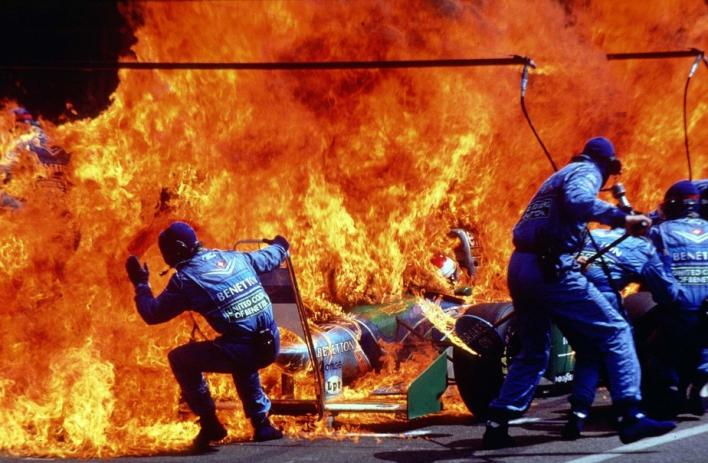
\includegraphics[height=150pt]{incendimento}
\caption{Carro de Jos Verstappen em chamas}
\label{fig:incendimento}
\end{figure}


\textbf{Esmagamento} -  Devido aos primeiros carros desenvolvidos para a \ac{f1} serem apenas focados em pura velocidade e em estabilidade, os responsáveis pelo desenvolvimento dos carros nunca se preocuparam com a segurança dos pilotos. Os carros eram equipados com as melhores peças mecânicas do momento, que eram capazes de produzir o máximo de potência, enquanto que o chassi seria o mais leve possível tendo a função de suportar as diversas partes do carro. Este conjunto resultava em um carro extremamente rápido, mas que deixava muito a desejar pois deixaria pouco espaço para o piloto, o que em caso de acidente faria com que este fosse esmagado pelas inúmeras partes que constituíam o carro;\\[0.5cm]

\textbf{Força G} - Todos nós já sentimos uma força que nos puxa no sentido contrário ao movimento que o carro faz quando este descreve uma curva. Essa força é designada por Força G sendo 1G o equivalente ao peso que o nosso corpo exerce sobre a Terra. Enquanto um piloto de \ac{f1} faz uma curva, este sente uma força que poderá atingir os 7G, o que poderá ser tolerável para um piloto tendo este preparação física prévia e realizando exercícios de respiração enquanto experiência estas forças assim como os pilotos de aviões de manobras rápidas.
Durante um acidente de carro um piloto pode experienciar dezenas ou em alguns casos, centenas de Gs o que pode resultar em lesões fatais ao piloto que acabará por ter uma morte instantânea na altura do impacto;\\[2.5cm]

A partir do ano de 1970 a \ac{fia} assumiu as rédeas em termos de proporcionar a melhor segurança possível para os seus pilotos. Conseguimos ver um aumento da consciência por parte dos responsáveis deste desporto, implementando novas medidas de segurança tais como:
\begin{itemize}
\item Uso de fatos (luvas, botas e roupa interior) à prova de fogo e calor;
\item Instalação do Cockpit rígido (desenvolvido para promover maior segurança ao piloto em caso de despiste);
\item Modificação da engenharia dos carros (modificação da disposição e das estruturas das peças que compunham o carro, reforçando grande parte delas para fornecer maior segurança ao piloto);
\item Implementação do Safety Car (\autoref{fig:safety-car}, carro que limita a velocidade de carros que permite uma maior segurança para a resolução de qualquer obstrução em pista);
\item Protocolos (conjunto de regras com objetivo a precaver futuros incidentes). 
\begin{figure}[h]
\center % Centra as imagens
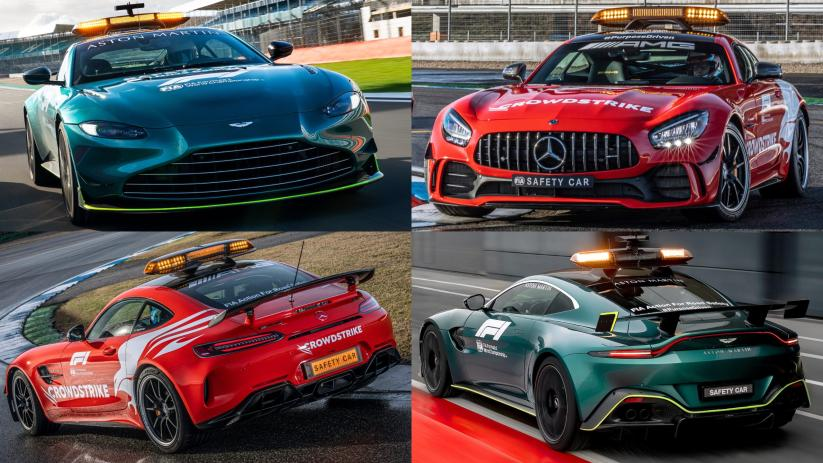
\includegraphics[height=150pt]{safety-car}
\caption{Formula 1 2021 Safety Car's}
\label{fig:safety-car}
\end{figure}

\end{itemize}

Até ao dia de hoje, desde que a \ac{fia} implementou este conjunto de regras, as mortes no desporto reduziram drasticamente passando de 17 a 3,4 por década. A última morte registada na \ac{f1} remete a 17 de Julho de 2015 onde o jovem Jules Bianchi de 25 se despistou e embateu contra um veiculo pesado que removia outro carro que havia sofrido outro acidente. Foi mais tarde revelado que Jules Bianchi sofreu uma lesão axonal difusa (quando o cérebro move-se violentamente no crânio) devido á repentina Força G a que foi submetido no impacto.



\chapter{Estado da Formula 1}
Muita coisa mudou desde que o primeiro Grande Prêmio do Campeonato Mundial de \ac{f1} foi realizado em Silverstone, no Reino Unido, no ano de 1950. Atualmente a \ac{f1} é, sem dúvida, o automobilismo tecnologicamente mais avançado do mundo. Para além disso, atualmente a \ac{f1} é um desporto mais seguro devido às implementações feitas pela \ac{fia}, que vieram trazer uma maior segurança aos pilotos, assim como uma maior competitividade entre eles. Ao longo da história deste desporto, poderemos ver algumas tecnologias desenvolvidas na \ac{f1}, serem utilizadas no mundo da viação civil.
\begin{figure}[h]
\center % Centra as imagens
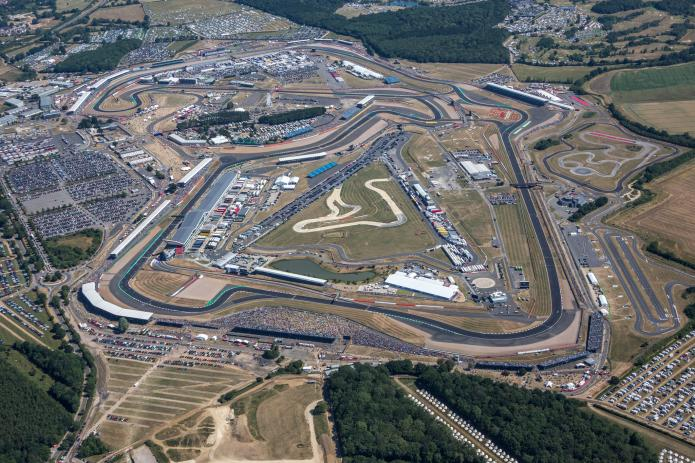
\includegraphics[height=200pt]{silverstone}
\caption{Silverstone, British Grand Prix}
\label{fig:silverstone}
\end{figure}

\chapter{Avanços Tecnológicos na Formula 1}
A \ac{f1} sempre foi principalmente conhecida pelos seus enormes riscos associados ao desporto. Atualmente, a \ac{f1} é um desporto muito mais seguro comparado ao seu primórdio, onde, já abordado anteriormente existiriam imensas mortes e feridos derivados dos acidentes. Não pela quantidade de acidentes ocorridos, mas sim pela falta de segurança no desporto.


Desde o seu primórdio até a atualidade a \ac{f1} evoluiu drasticamente, aprendendo com os seus erros que acabariam por deixar graves marcas no desporto. Tal evolução deveu-se aos grandes avanços tecnológicos que não só vieram trazer uma maior segurança para os pilotos, mas também uma competitividade mais apelativa e intensa quer para estes, quer para os seu fãs, através das seguintes novidades tecnológicas:

\section{Segurança}	

\begin{itemize}

\item \textbf{Halo} – Como poderemos ver na \autoref{fig:halo}, o Halo, também conhecido como auréola devido ao seu design único, é um sistema de proteção contra colisões, que consiste em uma barra curva feita em titânio, pesando 9 kg e suportando até 12 toneladas. Este, encontra-se fixado ao carro através de 3 pontos de contacto e, o seu design e material foram desenvolvidos e escolhidos com o objetivo de garantir a segurança dos pilotos. Até ao dia de hoje, o halo já salvou inúmeras vidas, sendo que o auge do seu reconhecimento ocorreu no Grand Prix de Bahrain de 2020, onde, o francês Romain Grosjean esteve envolvido em um acidente, onde, após ter embatido contra uma barreia de ferro a uma velocidade de 200 km/h, escapou com apenas queimaduras ligeiras nas suas mãos. 
No final deste GP, a \ac{fia} concluiu através da investigação realizado ao acidente, que sem o dispositivo de segurança Halo, o piloto teria sido imediatamente decapitado pela barreira.
\begin{figure}[h]
\center % Centra as imagens
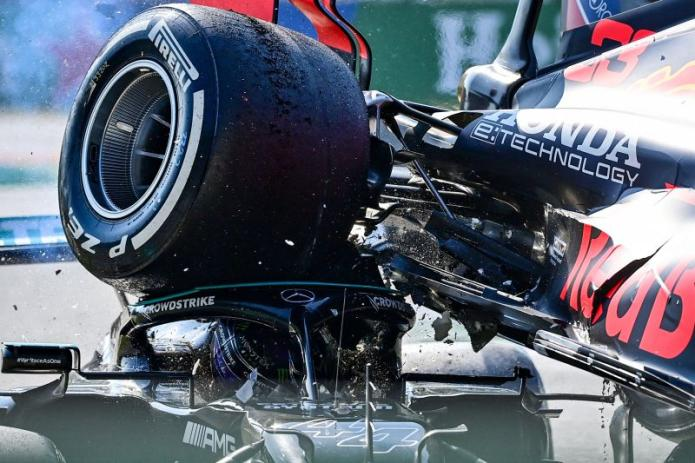
\includegraphics[height=150pt]{halo}
\caption{Halo}
\label{fig:halo}
\end{figure}

\item \textbf{Monocoque} – Como poderemos ver na \autoref{fig:monocoque}, o monocoque, também conhecido como célula de sobrevivência (Survival Cell), é o habitáculo onde se encontra os dispositivos de interação com o carro assim como o assento para o piloto. Constituído por várias camadas de fibra de carbono, esta, é a parte mais resistente do carro tendo como objetivo, garantir a segurança do piloto. Este, foi desenvolvido para ser praticamente indestrutível visto que, desempenha um grande papel na segurança do piloto.
Para garantir a segurança do mesmo, em circunstâncias extremas, o monocoque encontra-se programado para se separar do carro, de forma que o motor, parte elétrica e tanque de combustível fiquem longe do piloto, que possui um sistema de libertação rápida (Quick Release) para que possa abandonar rapidamente a célula.
No mesmo acidente onde podemos ver um breve exemplo da utilidade do Halo no GP de Bahrain de 2020, poderemos encontrar um excelente exemplo onde, o monocoque desempenhou um papel imprescindível, mantendo o piloto em segurança. 
O acidente contra as barreiras resultou em um impacto de 67 Gs que, automaticamente separou a célula da traseira do carro, o que deu tempo ao piloto para que conseguisse sair do seu habitáculo sem que as chamas o envolvessem de forma imediata.\\[4cm]
\begin{figure}[h]
\center % Centra as imagens
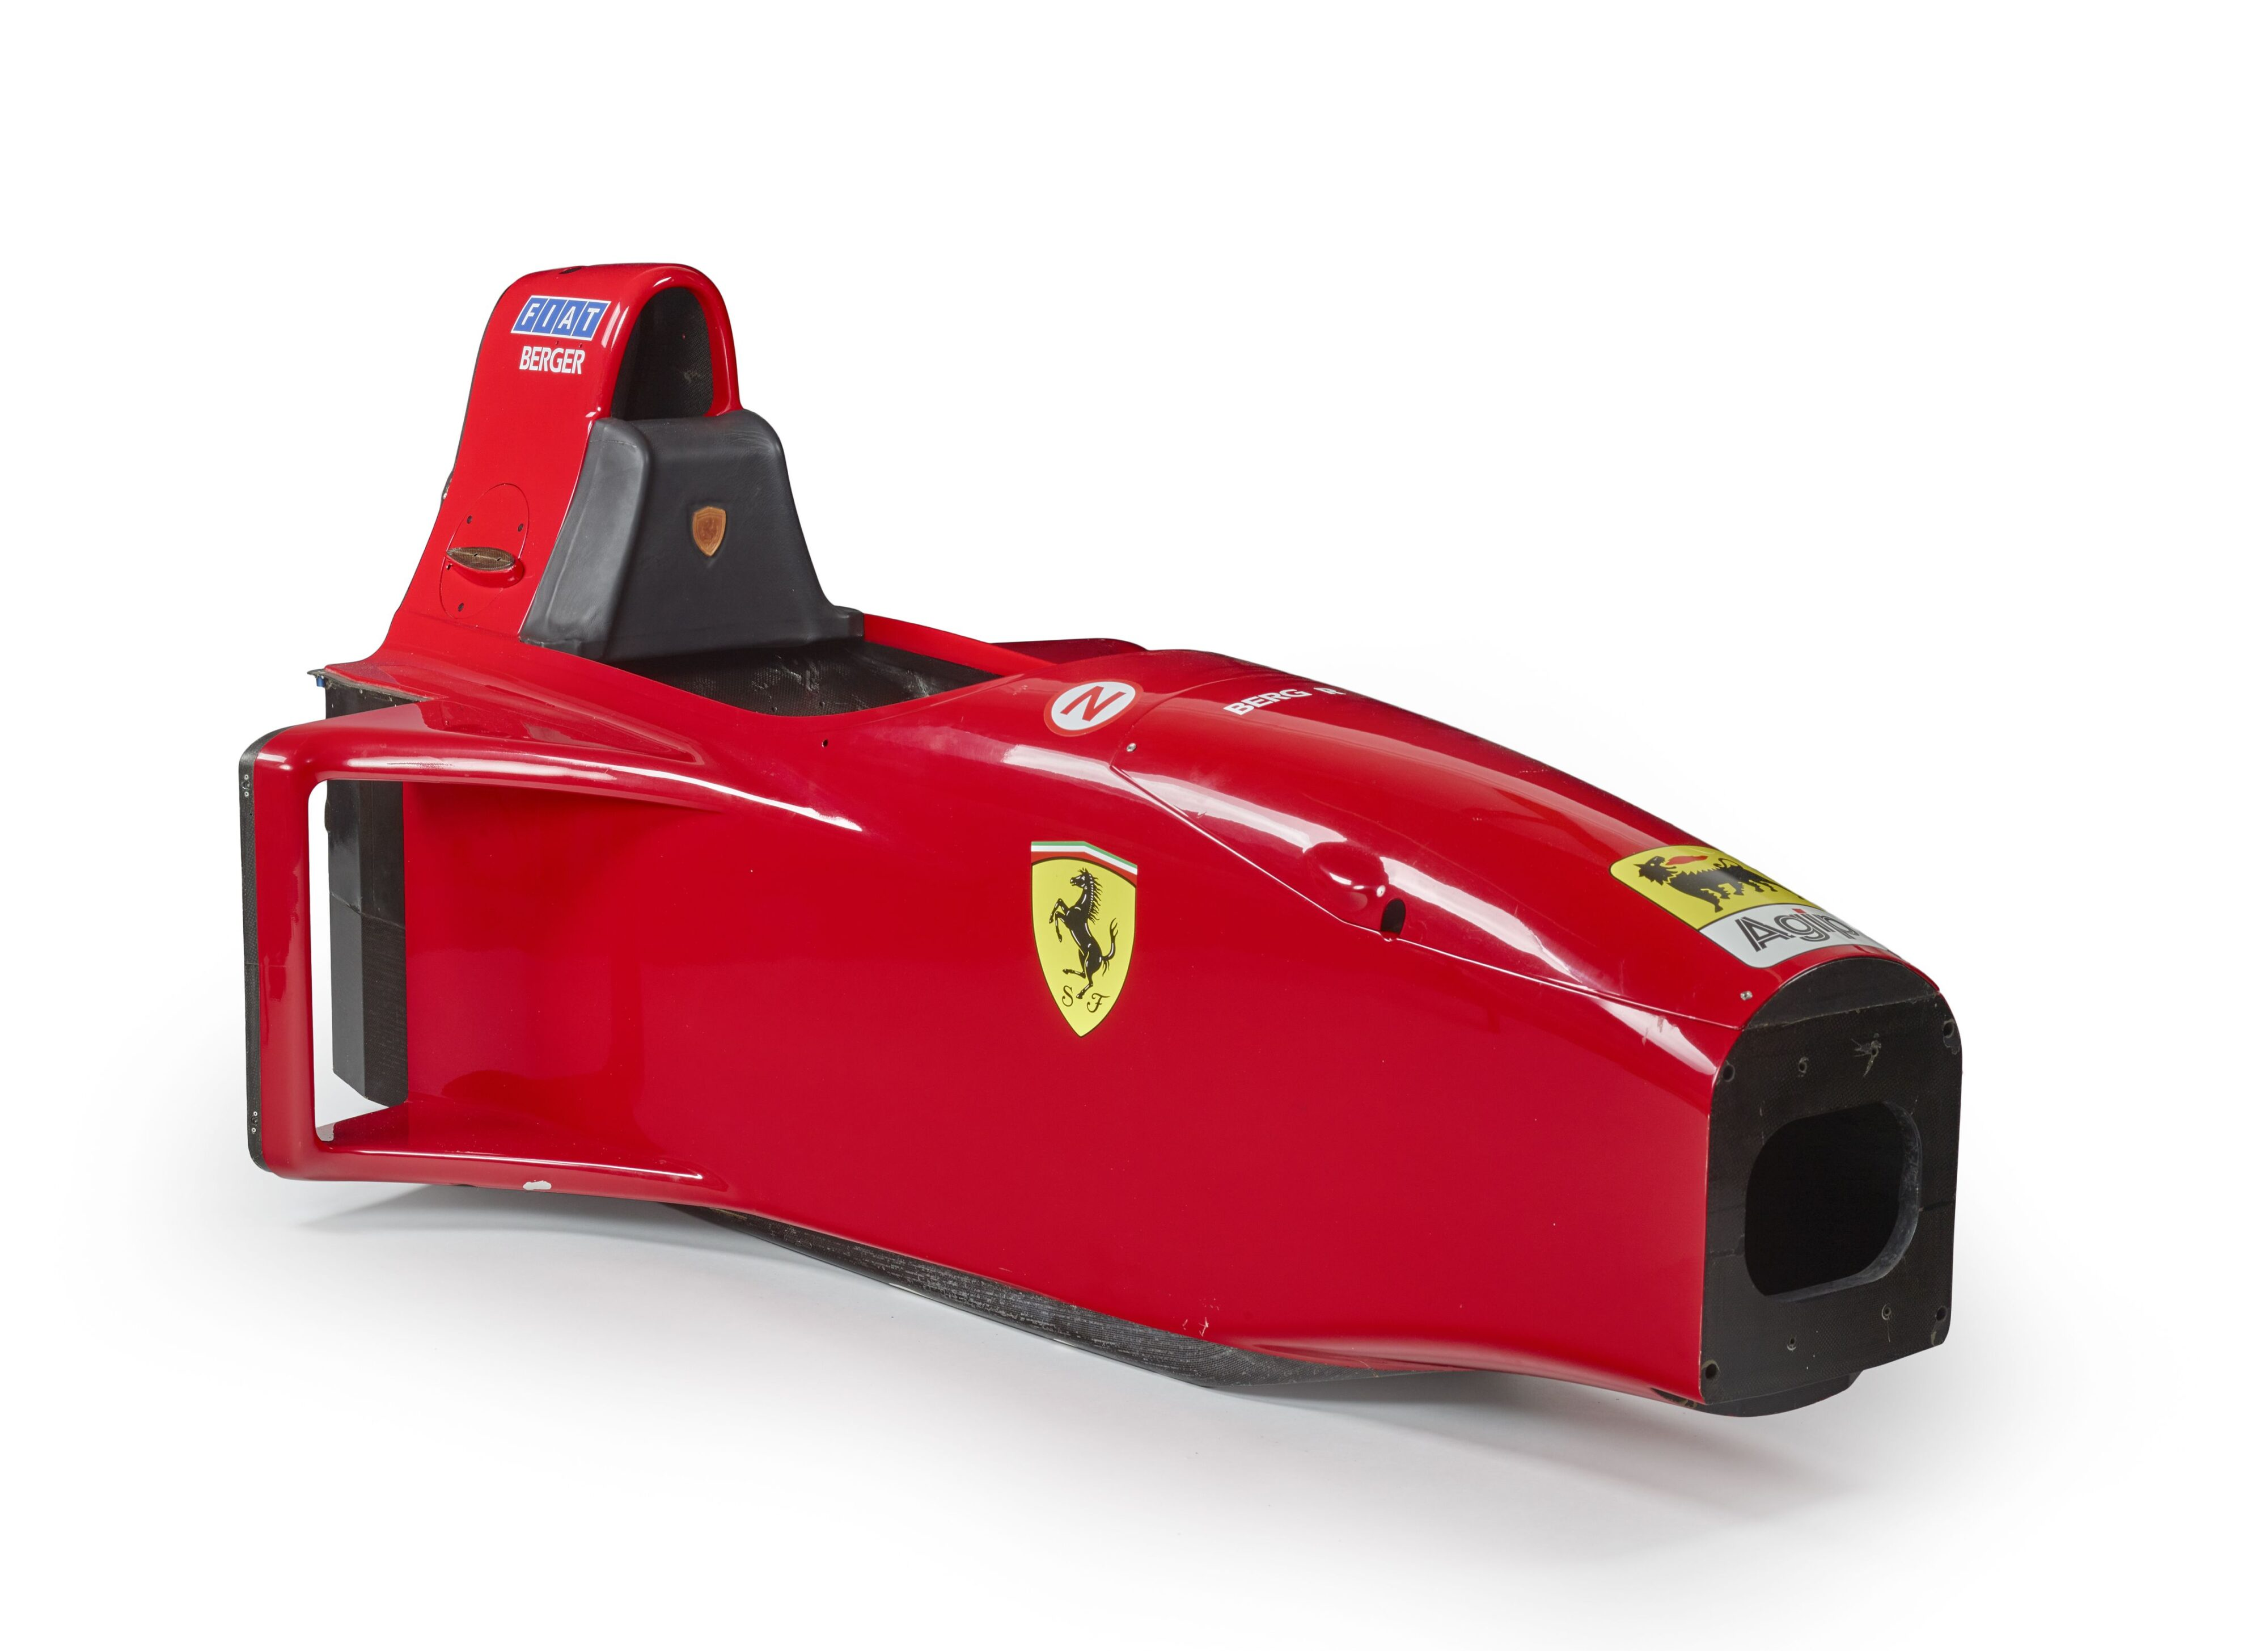
\includegraphics[height=150pt]{monocoque}
\caption{Monocoque}
\label{fig:monocoque}
\end{figure}


\item \textbf{Vestuário de corrida} – O vestuário de corrida na \ac{f1} é composto por sapatos, luvas, fato e capacete (\autoref{fig:vestido}). Todo o vestuário exceto o capacete, são produzidos utilizando dois tipos de tecido, Nomex e Kevlar. O Kevlar, protege os pilotos pois, é resistente a material perfurante, enquanto o Nomex é um tecido que quando exposto ao fogo, a uma temperatura de 370 graus celsius não degrada, derrete nem pega fogo. Quando exposto a 500 graus, este tecido começa a degradar-se, mas ao contrário dos outros tecidos, este transforma-se em carbonáceos que acaba por funcionar como um isolante térmico que suporta temperaturas até 900 graus.
Os capacetes dos pilotos são constituídos por várias camadas de Kevlar, fibra de carbono e polietileno. Estes são capazes de resistir a temperaturas superiores a 800 graus e objetos projetados a mais de 500 km/h. Enquanto o exterior do capacete é projetado para ser rijo e resistir a grandes impactos assim como a altas temperaturas, o interior tem a responsabilidade de dissipar a energia para evitar desacelerações bruscas assim como em caso de incêndio, manter uma temperatura interior inferior aos 70 graus.
Desde o ano de 2019, as luvas utilizadas pelos pilotos contêm sensores biométricos cosidos no tecido como poderemos ver na \autoref{fig:luvas}, com, que monitoriza a pulsação e a quantidade de oxigénio no sangue.
Mais uma vez, com o exemplo do acidente do piloto Romain Grosjean no GP de Bahrain 2020, poderemos ver uma utilização desta tecnologia onde, após ter colidido com a barreira, a pulsação e a oxigenação do piloto foi imediatamente monitorizada através destas luvas que desempenham um papel vitalício ao fornecer informação sobre o estado dos pilotos.\\[1.5cm]


\end{itemize}

\begin{figure}[h]
\center % Centra as imagens
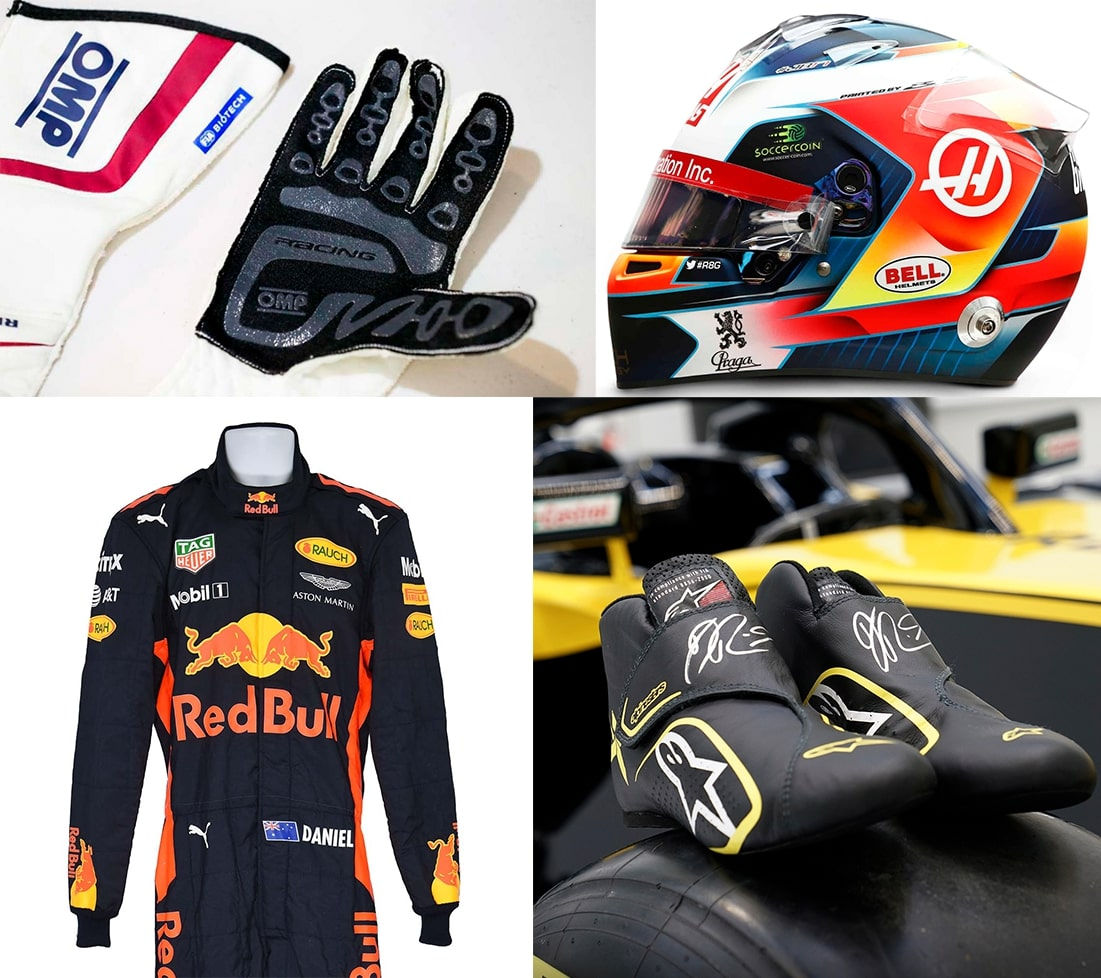
\includegraphics[height=250pt]{vestido}
\caption{Vestuário usada na \ac{f1}}
\label{fig:vestido}
\end{figure}


Tendo em conta os dispositivos de segurança e os seus respetivos avanços tecnológicos apresentados, podemos concluir que todos estes dispositivos juntos, vieram trazer uma segurança altamente qualificada para o desporto pois, quando estes realizam a função pela qual foram concebidos, trazem com eles uma maior segurança para os pilotos. Como podemos ver, todos estes dispositivos estiveram presentes e realizaram o seu papel no acidente de Romain Grosjean, evitando assim mais uma fatalidade para o desporto e, tornando o piloto numa testemunha viva do quão seguro a \ac{f1} veio a ser.
	
\section{Competição}

\begin{itemize}

\item \textbf{Asa Frontal} – A Asa Frontal (Front Wing, \autoref{fig:carro}) é uma parte crucial no carro pois, é o primeiro contacto que este tem com o fluxo de ar. A função da Asa é originar downforce que consiste em criar uma corrente de ar mais rápida debaixo do carro que fisicamente acaba por se traduzir numa força de sucção existente entre o carro e o chão, assim como numa força exercida nos pneus frontais que irá permitir ao piloto realizar as curvas com uma maior velocidade e perícia.
As Asas Frontais são constituídas por fibra de carbono e conseguem suster centenas de quilos. Estas, também têm como objetivo direcionar o fluxo de ar para arrefecimento dos travões frontais, assim como o motor e permitir uma melhor aerodinâmica que favoreça o design do carro.

\item \textbf{Asa Traseira} - A Asa Traseira (Rear Wing, \autoref{fig:carro}) tem como principal função aplicar força nos pneus traseiros para que haja um melhor atrito entre estes e o solo. Uma Asa maior será utilizada em circuitos com mais curvas e resultará em uma força maior, assim como uma Asa menor será utilizada em circuitos com um maior número de retas pois resultará em uma força menor aplicada sobre os pneus traseiros. Isto, dará ao piloto um melhor desempenho durante as retas e uma maior aderência nas curvas.  Tal como a Asa Frontal, a Asa Traseira também é constituída por fibra de carbono, capaz de suportar centenas de quilos.

\item \textbf{Difusor} – O Difusor (Difuser, \autoref{fig:carro}) permite maior competitividade entre pilotos, ofercendo ao mesmo tempo benefícios para quem o usa. A função do difusor tem como objetivo guiar o ar que circula por baixo do carro de forma a organizar o fluxo de ar impedindo que este saia do veículo de forma brusca e perturbada que acabará por trazer instabilidade para a traseira do carro. Caso um carro não esteja equipado com um difusor, os pilotos que o seguem terão uma tremenda desvantagem visto que a aerodinâmica dos carros de \ac{f1} está projetada para correr em ar em repouso (ar limpo).\\[0.7cm]

\item \textbf{DRS} – O \ac{drs} (\autoref{fig:carro}) tem como objetivo reduzir o arrasto criado pela asa traseira dos carros nas retas, o que, irá trazer ao carro uns 20 km/h a mais que os seus oponentes, o que resulta em uma corrida mais apelativa para os fãs com inúmeras ultrapassagens e mais competitivas para os pilotos com oportunidades de vantagem. O \ac{drs} apenas pode ser ativo nas zonas autorizadas em cada circuito e, se o oponente se encontrar a 1 segundo de alcance do piloto. Após um Safety Car o \ac{drs} fica desativado durante 2 voltas.

\item \textbf{ERS} – O \ac{ers} (\autoref{fig:carro}) consiste em recuperar a energia perdida pelo carro. Esta energia pode ser obtida através de 2 métodos, energia térmica e cinética. Para a energia térmica é utilizado um motor gerador térmico (MGU-H) enquanto para a energia cinética é utilizado um motor gerador cinético (MGU-K). A eletricidade gerada por esses motores é guardada numa bateria chama Energy Store (ES).
Quando um piloto se encontra a carregar as suas baterias, podemos deparar-nos com uma luz vermelha a piscar na sua Asa Traseira.
O piloto pode utilizar a energia sempre que assim o desejar, mas, a forma mais comum de o fazer é utilizando ou para atacar ou para defender da posição de um adversário. Quando o piloto ativa o \ac{ers}, este gera 120 Kw de potência extra.

\item \textbf{DAS} – O \ac{das} (\autoref{fig:carro}) consiste em alterar o ângulo em que os pneus estarão apontados para a frente (Toe In e Toe Out). O piloto poderá modificar o ângulo movendo a coluna de direção do seu carro para a frente ou para trás. Este sistema trouxe inúmeras vantagens pois permitiria o aquecimento rápido e uniforme dos pneus que acabaria por resultar em uma maior aderência. O \ac{das} permite realizar curvas em um raio menor e com uma velocidade maior que o normal.
Este sistema foi descoberto por parte da \ac{fia} em 2020, após ter sido usado durante algum tempo de forma secreta pela equipa Mercedes-Benz pois, viria a trazer-lhes uma vantagem sobre os seus adversários. Após a \ac{fia} ter descoberto este sistema, imediatamente baniu a descoberta pois a equipa pioneira estaria a ter uma vantagem gigantesca e principalmente, porque esta não respeitava para com o regulamento imposto pela \ac{fia}. \\[1cm]

\begin{figure}[h]
\center % Centra as imagens
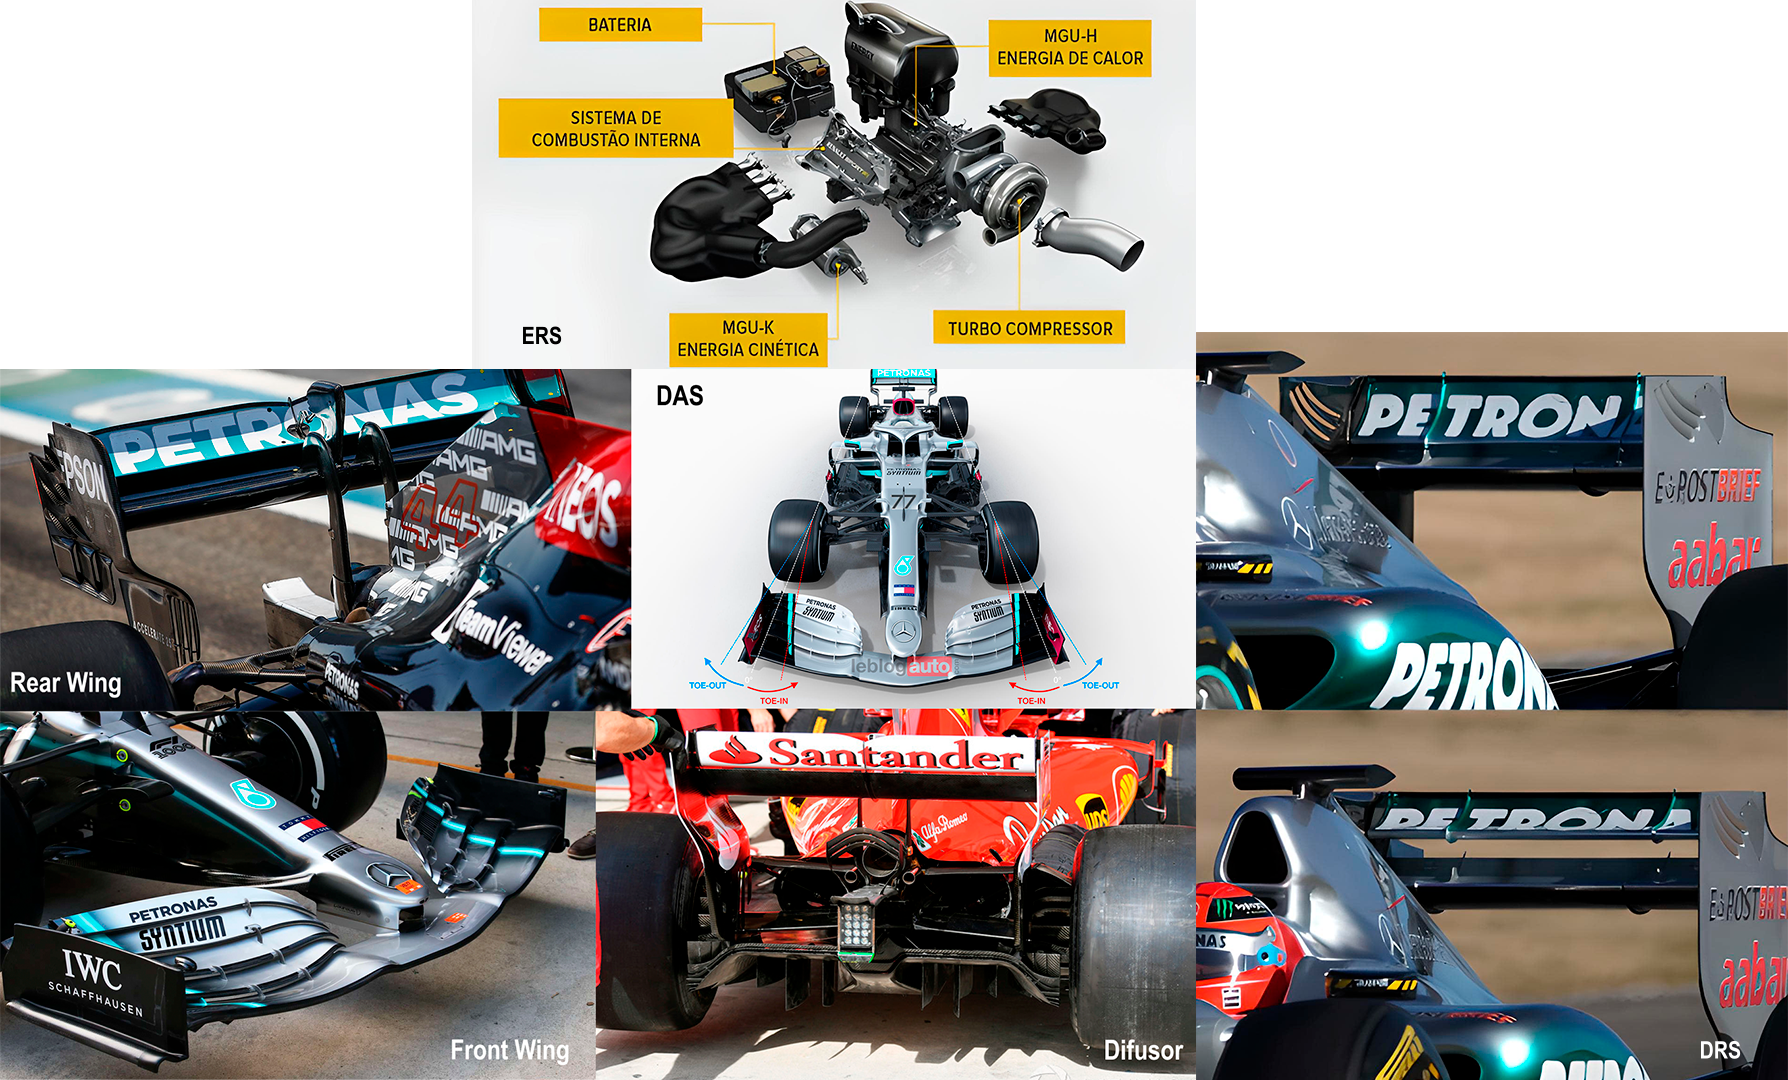
\includegraphics[height=250pt]{carro}
\caption{Rear Wing - Front Wing - DAS - Difusor - DRS - ERS \ac{f1}}
\label{fig:carro}
\end{figure}

\end{itemize}

\chapter{Formula 1 nos automóveis}
Desde o início da \ac{f1}, foram desenvolvidas inúmeras tecnologias que mais tarde acabariam por ser utilizadas no mundo da viação civil. Atualmente poderemos encontrar inúmeras dessas tecnologias presentes nos nossos automóveis sem sequer nos apercebermos, sendo a mais recente, a produção de peças em impressoras 3D. A produção de peças a partir de impressoras 3D deve-se ao seu reduzido gasto económico e à sua extrema precisão ao serem produzidas, o que por sua vez resulta numa menor despesa e num aumento da segurança da produção dos automóveis por parte da indústria automóvel.


Além desta já mencionada, existem outras tecnologias criadas da mesma forma que esta que, ao longo dos anos se tornaram mais acessíveis e, por sua vez poderemos encontrá-las atualmente nos nossos veículos diários.
Algumas dessas tecnologias são:
\begin{itemize}

\item \textbf{Spoilers} - Os Spoilers (\autoref{fig:carro2}), tal como na \ac{f1}, são utilizados para exercer mais força sobre os pneus traseiros, oferecendo assim uma melhor tração;

\item \textbf{Volantes Multifuncionais} – Este tipo de volantes (\autoref{fig:carro2}) passou a ser utilizado nos carros comuns pois, o condutor usufrui de várias funcionalidades no volante sem ter de se distrair procurando pelos mesmos;

\item \textbf{Caixa de Velocidade Automática} – Ao contrário dos carros com velocidades manuais, os carros com velocidades automáticas dispõem de um grande benefício pois não terão de pressionar na embraiagem para selecionar outra velocidade o que acaba por reduzir o risco de acidente. As mudanças num carro automático, podem ser selecionadas automaticamente pelo veículo ou fisicamente pelo condutor através de duas patilhas (borboletas, \autoref{fig:carro2}) que se encontram atrás do volante.

\item \textbf{Sistema de Recuperação de Energia} – Atualmente este sistema apenas se encontra nos carros mais caros visto que acaba por ser uma tecnologia recentemente desenvolvida na \ac{f1}, onde se designa por \ac{ers}. 

\item \textbf{Travões de Carbono} – Tal como o \ac{ers}, os travões de carbono (\autoref{fig:carro2}) são apenas utilizados nos carros mais caros, mas, cada vez mais se começa a ver a sua utilização em carros de classe média. Atualmente, os discos são feitos de fibra de carbono, o que ainda acaba por ser um material cuja produção é bastante dispendiosa, daí apenas serem vistos em carros de classe alta e média.\\[1cm]

\begin{figure}[h]
\center % Centra as imagens
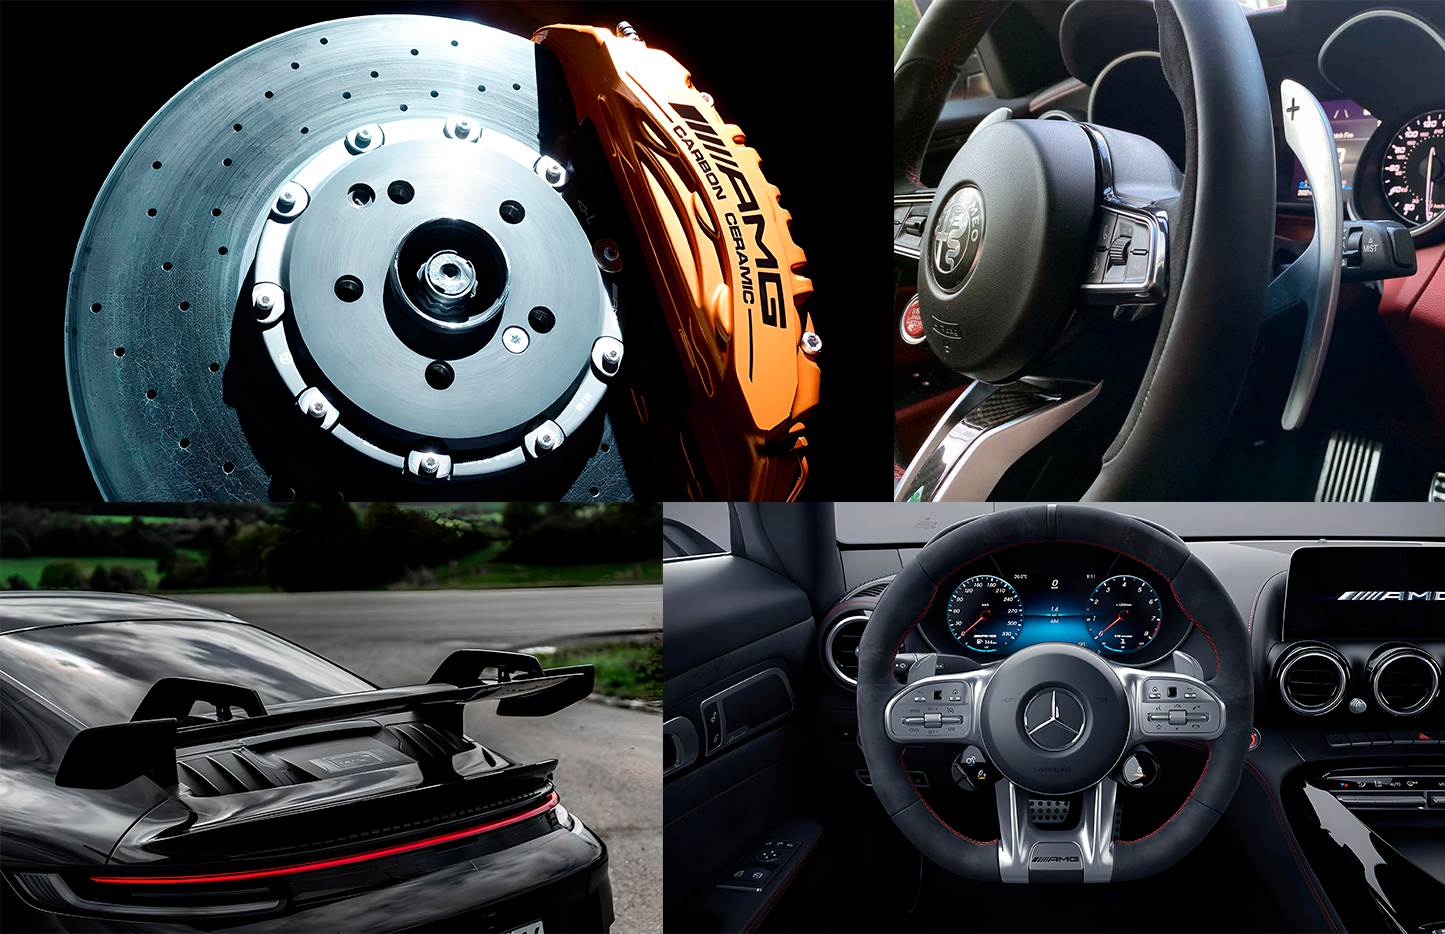
\includegraphics[height=230pt]{carro2}
\caption{Spoiler - Volante Multifuncional - Borboletas - Travão de Carbono}
\label{fig:carro2}
\end{figure}

\end{itemize}

\chapter{Conclusão}
Em suma, respondendo á pergunta inicialmente feita neste projeto, poderemos concluir que a \ac{f1} evoluiu bastante ao longo deste 71 anos, destacando-se a preocupação pela segurança dos pilotos e, por isso mesmo, a \ac{fia} adotou medidas importantes para a segurança destes mesmos. Para além disso, a \ac{f1} evoluiu também a nível tecnológico, de forma que este, continuasse a ser um desporto competitivo e apelativo. Por consequente, a \ac{f1} teve um impacto colossal no mundo da viação civil melhorando a segurança nos automóveis e a comodidade destes. Do que poderemos esperar da \ac{f1} no futuro, é decerto que este magnifico e competitivo desporto, irá continuar a evoluir e a influenciar na produção dos carros no mundo da viação civil.

\chapter{Contribuições dos autores}

Os seguintes capítulos foram realizados por \ac{bf}:
\begin{itemize}
\item História da Formula 1
\item Estado atual da Formula 1
\item Introdução/Conclusão
\item Resumo\\[0.5cm]
\end{itemize}

Os seguintes capítulos foram realizados por \ac{tf}:
\begin{itemize}
\item Segurança no primórdio da Formula 1
\item Avanços Tecnológicos na Formula 1
\item Formula 1 nos Automóveis
\item Realizar Projeto em Latex\\[0.5cm]
\end{itemize}

\ac{bf} - 50\%


\ac{tf} - 50\%


%%%%%%%%%%%%%%%%%%%%%%%%%%%%%%%%%
\chapter*{Acrónimos}
\begin{acronym}
\acro{ua}[UA]{Universidade de Aveiro}
\acro{miect}[MIECT]{Mestrado Integrado em Engenharia de Computadores e Telemática}
\acro{lei}[LEI]{Licenciatura em Engenharia Informática}
\acro{glisc}[GLISC]{Grey Literature International Steering Committee}
\acro{bf}[BF]{Beatriz Ferreira}
\acro{tf}[TF]{Tomás Fonseca}
\acro{fia}[FIA]{Federação Internacional de Automobilismo}
\acro{f1}[F1]{Formula 1}
\acro{drs}[DRS]{Drag Reduction System}
\acro{ers}[ERS]{Energy Recovery System}
\acro{das}[DAS]{Dual Axis Steering}
\end{acronym}


%%%%%%%%%%%%%%%%%%%%%%%%%%%%%%%%%
\printbibliography

\end{document}
